Program comprehension is a concept of understanding code to perform different software maintenance tasks. In recent years, the size of the code base is increasing drastically, which makes program comprehension difficult. To cope with the demand, many research works have been performed to understand how developers comprehend a program or code snippet and how to support developers to start their assigned tasks quickly. Different cognitive models are proposed in the literature to ease comprehension. 
Recently, studies to cluster execution paths of a call graph to aid overall program comprehension are going on.
We argue that this structure can be used to aid the top-down and bottom-up cognition model of program comprehension.
This paper has adopted new techniques for the hierarchical abstraction of a software system that performs better than the existing literature's related techniques. We conducted an exploratory case-study with three subject systems to validate our hypothesis. We found that it is possible to use this hierarchical presentation to enrich above mentioned cognition models.   

\section{Introduction}

One of the crucial parts of a software engineering job is software maintenance. Four types of software maintenance task are perfective, preventive, corrective, and adaptive \cite{williams2010characterizingArchitectureChanges}. To perform all of these tasks, developers first need to understand the target system, how its different components work together, and locate the relevant classes, methods, and files for completing a specific task. To add or change something in the system accurately and adequately, developers need to understand how its different components work together and map the implementation level source code to high-level features. Proper tool support for program comprehension can reduce the manual and economic cost of software maintenance, which will result in cheaper software \cite{arisholm2006impactUMLDocumentation}. In the literature, the studies on program comprehension are divided into two parts \cite{levy2019understandingLargeHierarchical}. First, how developers understand a code snippet. Second, understanding how large software systems are comprehended. Levy et al. \cite{levy2019understandingLargeHierarchical} conducted a study to find how comprehending a large system works from an experienced developer's perspective. The comprehension of a system has a conceptual and concrete level \cite{bass2003softwareArchitecturePractice, levy2019understandingLargeHierarchical}. In reverse software engineering, different tools are used to extract implementation level architecture from source code (call graph). Later, through manual analysis, they are mapped to concept level architecture, which helps cognitive mapping \cite{roy2008softwareArchitectureRecovery}. However, as software systems are getting more complex in size, manual analysis of implementation level architecture to high-level concepts requires more human resources. In most cases, they are exhausting. 

Studies on processing call graphs to facilitate overall system comprehension are very common in literature \cite{cornelissen2007understandingMassiveSequence, feng2018hierarchicalExecutionComprehension, reiss2005dynamicSoftwarePhases, watanabe2008featurePhaseDetection} . The dynamic call graph is used for most studies, which is good for specific test cases or scenarios. The problem with the dynamic call graph is they have redundancy problems and cannot capture the whole software systems \cite{gharibi2018automaticStaticCluster}. Recently research on overall system comprehension focused on static call graph took attention \cite{gharibi2018automaticStaticCluster, walunj2019graphevoEvolutionCall}. Execution paths from static call graphs \cite{pradel2009automaticUseageSpecification, salah2005scenariographerReverseEngineering} can be used to extract usage scenario or high level functionality. Clustering execution paths from both static and dynamic call graph pave the way for the hierarchical abstraction of the system \cite{feng2018hierarchicalExecutionComprehension, gharibi2018automaticStaticCluster}. Labeling these intermediate nodes of a cluster tree can create a hierarchical abstraction tree with concepts as the label. We argue that this type of tree representation can aid developers in using different program comprehension models. For example, the Bottom-up model is used by developers when they do not have any knowledge about the domain of the system. They gradually try to map low-level properties to high-level concepts. Developers can use the cluster tree of execution paths to facilitate Bottom-up cognition. The clustering starts from execution paths (low-level features) to a gradual grouping of similar paths, which are high-level features. Similarly, the cluster tree can help automate the top-down cognition model. 

In the top-down model, when developers have domain knowledge of a system, they try to map the knowledge to low-level implementations. The cluster tree hierarchically abstracts the features so that we have domain knowledge at the top of the tree that we can relate to low-level features by browsing the tree in a top-down manner. From our manual investigation to the proposed approach of Gharib et al. \cite{gharibi2018automaticStaticCluster}, we found that the abstraction tree has the potential to support program comprehension models automatically. However, they only used top-5 function names from the execution paths as the intermediate abstraction node label. We found that labeling the abstraction node properly with supporting documentation and example can make the hierarchical abstraction tree more attractive and comprehensive to the developers. This paper has proposed three techniques to improve the abstraction of intermediate nodes in a cluster tree. 

\begin{itemize}
    \item First, we experimented with labeling the nodes using TFIDF, LDA, and LSI information retrieval techniques. Previous studies only used the TFIDF technique.
    \item Second, we generated natural text descriptions for each node by summarizing comments from the execution paths' methods.
    \item Third, inspired by Feng et al. \cite{feng2018hierarchicalExecutionComprehension}, for each node, we attached significant patterns from execution paths by applying Sequential pattern mining. To validate our techniques, we conducted an exploratory case study with three subject systems to find how these techniques can automatically help developers in program comprehension. 
\end{itemize}

Our investigation shows that providing a natural text description and sample execution patterns increase the comprehensibility of abstraction nodes. 
  
The rest of our paper is organized as follows. In section \ref{motive}, we discussed the potential of the proposed approach by analyzing a sample calculator program. Section \ref{approach} describes how the proposed approach works. In Section \ref{related}, a brief discussion of existing relevant works is presented. In Section \ref{evaluation}, an exploratory case study is reported to validate our proposed techniques.

\section{Motivational Example}
\label{motive}
To demonstrate how a software system's hierarchical abstraction will work, we have created a sample Calculator program. The program takes two numbers as input, validates the inputs, and prompts the user to input which operations they want to perform. Later, according to the input, addition, subtraction, multiplication, division can be performed. This is a brief functionality of the calculator program. 


In Figure \ref{fig:motivation} we have presented the hierarchical abstraction of the Calculator program. From the figure, we can see our Calculator program has six execution paths. Their node number is from 0-5. 
\begin{itemize}
    \item Execution path 0 and 1 represent the functionality of multiply two numbers and adding two numbers, respectively. For these two clusters, add and multiply is the two different job they are doing. Other functions of the two paths are similar. So, the abstraction of these two execution paths is Intermediate node 7. Five keywords are picked as the abstraction of execution paths 0 and 1. From the keywords of node 7, it is clear that descendent nodes do addition and multiply on two numbers.
    \item Next, for node 10, we can see the keywords are add, divide, mod, multiply, and subtract. These five keywords indicate that the descendant nodes of 10 do these numerical operations. If we observe the five execution paths (EP 0 - 4), we find that they perform add, delete, mod, multiply operation on two input numbers. We can see that the five keywords of node 10 summarize the functionality of its descendants.
    \item Similarly, for node 11, the keywords are mod, multiply, subtract, valid, and number. We can see the right child node (node 5) of node 11 input two numbers and then validates it. Left descendants of node 11 perform numerical operations. So, the summary of node 11 contains three words relevant to operation and two for input validation.
\end{itemize}
   From our understanding, we can see that this is an almost human level summary for node 10. The summary presented in Figure \ref{fig:motivation} is generated using Tfidf score on words in method name. This figure can help both top-down and bottom-up cognition model of program comprehension to explore the Calculator program. To further assist this purpose, we also provided a text description of the nodes (by summarizing comments of methods) and a glimpse of the execution paths' inside by mining sequential patterns.  
\begin{figure*}[tb]
  \centering
  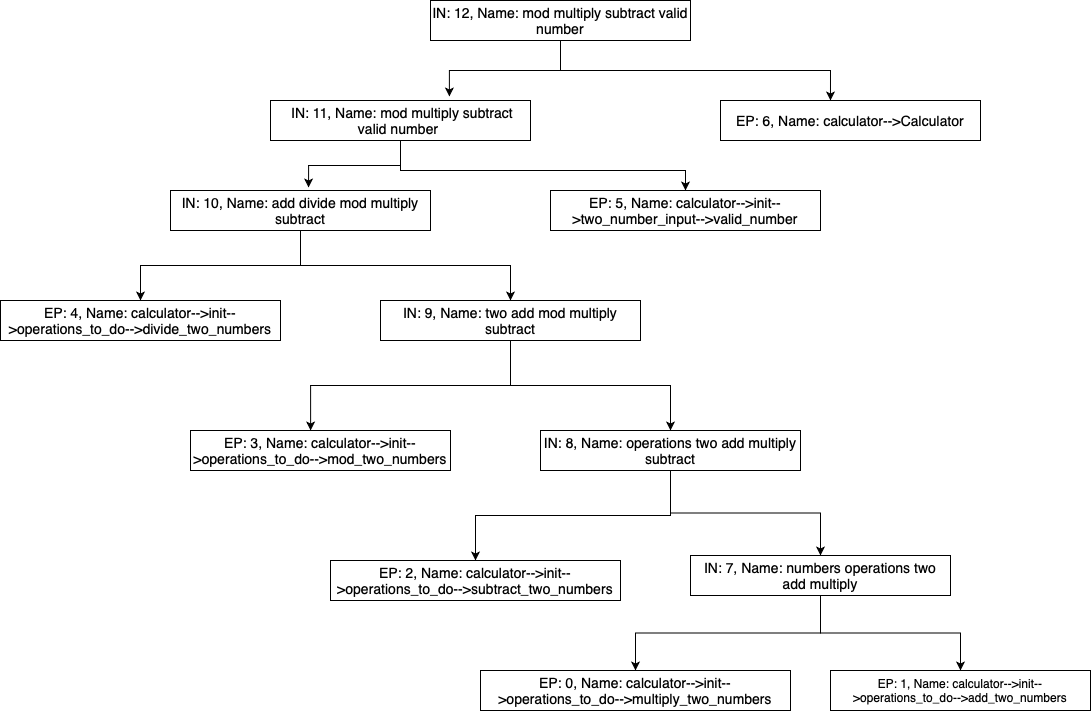
\includegraphics[width=\columnwidth]{figures/hla2/motivation_n.png}
  \caption{Hierarchical abstraction of the calculator program (EP means Execution path or leaf node and IN means Hypothetical abstraction or Intermediate Node)}~\label{fig:motivation}
\end{figure*}

\section{Approach}
\label{approach}
\begin{figure*}[tb]
  \centering
  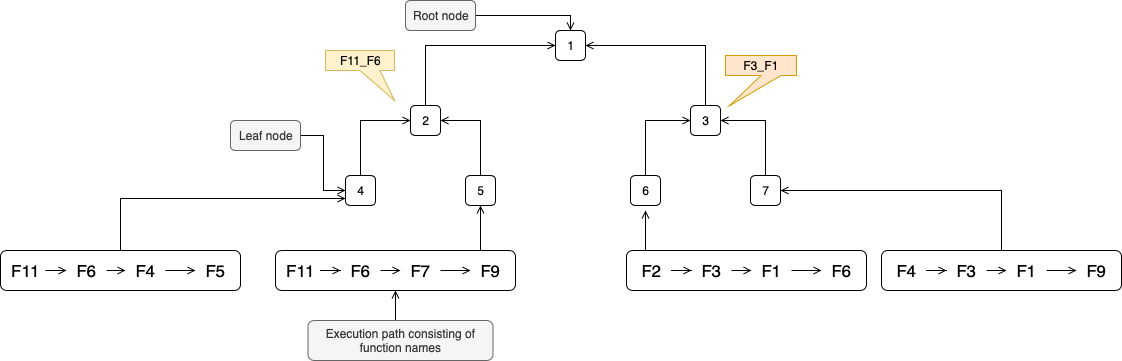
\includegraphics[width=\columnwidth]{figures/hla2/tree_structure.png}
  \caption{Structure of a hierarchical abstraction tree}~\label{fig:tree_structure}
\end{figure*}
In this section, we discuss two significant steps in our approach with a brief discussion. First, we described six steps to get the subject system's hierarchical abstraction tree in Section III-A. Second, in Section III-B, we describe how we used different information retrieval techniques to define the tree's hypothetical abstraction nodes. Data collection for evaluating the approach is depicted in algorithm \ref{alg:overall}.


\begin{algorithm}
    \SetKwInOut{Input}{Input}
    \SetKwInOut{Output}{Output}
    
    \underline{Call Graph to Concept Cluster Tree} $(call graph)$\;
    
    \Input{Call graph}
    \Output{Concept cluster tree}
    \For{Iterate each node in the call graph}
    {
        \If{ $Number\_of\_Incoming\_Degree(node) == 0$}
        {
            entryNodes.append(node);
        }
        \If{$Number\_of\_Outgoing\_Degree(node) == 0$}{
            exitNodes.append(node);
        }
    } 
    \For{$i\gets1$ \KwTo $entryNodes.length$ \KwBy $1$}
    {
        \For{$j\gets1$ \KwTo $exitNodes.length$ \KwBy $1$}
        {
            execution\_paths.append($simple\_DFS\_path(i, j)$)
        }
    }
    \For{$i\gets1$ \KwTo $execution\_paths.length$ \KwBy $1$}
    {
        \For{$j\gets1$ \KwTo $execution\_paths.length$ \KwBy $1$}
        {
            $distance\_matrix[i][j]$ = $consine\_similarity(i,j)$;
        }
    }
    $cluster\_tree$ = $create\_cluster\_tree(distance\_matrix)$;
    
    $hierarchical\_abstraction\_tree$ = $label\_clusters(cluster\_tree)$;
    
    return $hierarchical\_abstraction\_tree$;
    \caption{Our procedure for analyzing Python source code of a project to construct concept cluster tree}
    \label{alg:overall}
\end{algorithm}

% \vspace{4mm}
\subsection{Hierarchical abstraction tree of a software system}
A call graph is a visual representation of a software system's method invocation relationships between different methods. We adopted a static call graph, which is generated by analyzing source code. As a static call graph captures whole function calls of a target system, we choose to abstract the target system. Previous studies suggested that function names contain significant abstraction of source code. 
Thus, we emphasized mining keywords by analyzing function names in the static call graph.
As we wanted to abstract the whole system's high-level functionality hierarchically, therefore the decision to adopt the static call graph as a building-block of our approach is well-justified.

In Figure \ref{fig:tree_structure}, we presented the hierarchical abstraction tree structure. The leaf nodes of this tree are directly mapped to the execution paths. Execution paths are a list of function names executed sequentially during the execution of a software system. For instance, node 5 is mapped to the execution path where F11, F6, F7, and F9 are called sequentially. 
In this scenario, all the leaf nodes (4, 5, 6, 7) are mapped to four execution paths or function call sequences.
Node 1, 2, and 3 are hypothetical abstractions of the four leaf nodes.
Generating meaningful descriptions for these intermediate nodes can make the abstraction tree helpful towards different program comprehension cognition models.
In the figure, nodes 2, 3 have been labeled F11\_F6, F3\_F1, respectively. These labels are generated by analyzing their child nodes' function names. We plan to generate five keywords for each intermediate node, alongside a short natural text description (from the doc-string of function names) and few significant patterns from analyzing execution paths under investigation.

\begin{figure*}[tb]
  \centering
  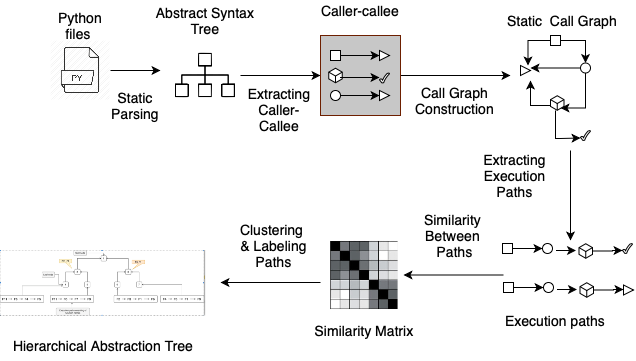
\includegraphics[width=\columnwidth]{figures/hla2/approach_new.png}
  \caption{Overview of the overall approach}~\label{fig:overall}
\end{figure*}

\subsubsection{Analyzing source code using modified Pyan module}

We used a modified version of Python module Pyan \cite{pyan} to extract function relationships from a Python system. Pyan works only for a single directory. We adapted Pyan so that it can consider multiple directories while extracting the relationships. Pyan uses the AST tree for extracting function relationships. After analyzing the source code, we generated a graph in TGF format (Trivial Graph Format). In TGF format, all modules and functions' physical addresses in the source code are printed first. Then, relationships between all functions are presented as the caller and callee pair.

\subsubsection{Extracting function relationships from Trivial graph format}

Function relationships from the TGF file format are used as inputs in our technique. Encoded unique identifiers are used to replace function names for ease of processing during the hierarchical clustering step.

\subsubsection{Static call graph creation based on the extracted relationships}
To perform different graph operations, we have created graph objects of NetworkX \cite{networkx} module using the extracted function relationships. 
\subsubsection{Extracting execution paths}

The execution path is a simple path between an entry node and an exit node. An entry node is a node in the call graph which incoming edge degree is zero. So, no function is dependant on an entry node. An exit node is a node that has a zero degree of outgoing function calls. We have generated a list of entry and exit nodes to generate execution paths from a call graph. Simple Paths calculation algorithm of the NetworkX \cite{networkx}  is used in our approach, which applies the \texttt{DFS} algorithm to get the paths between a source node and a destination node. For our task, a source node is an entry node, and a destination node is an exit node.    

\subsubsection{Distance matrix for execution paths}

For clustering execution paths (sequence of function names), we need to measure the similarity between all pairs of execution paths. For this purpose, we  \cite{niwattanakul2013jaccardKeywordsSimilarity} implemented the Jaccard similarity measure. The linkage algorithm uses this similarity in the next step. If we have two sets $A$ and $B$, then their Jaccard similarity will be the ratio of the cardinality of their intersection by the union. As clustering algorithm works on distance in our case dissimilarity between two execution paths/clusters, we have subtracted the similarity score with one to get the dissimilarity value according to equation \ref{eq:jaccard}. After calculating dissimilarity between all pairs of execution paths, we converted the 2d matrix to 1d condensed matrix to make our program memory efficient.

\begin{equation}
Dis(A, B) = 1 - \frac{A\cap B}{A\cup B}
\label{eq:jaccard}
\end{equation}

\subsubsection{Clustering execution paths using linkage algorithms}

To group similar execution paths as clusters, we have implemented a linkage algorithm using the popular Python package Scipy \cite{scipy}. Scipy has a lot of different types of linkage algorithms already implemented in its core. To update the distance between two clusters, we have picked the Ward \cite{ward} minimum variance method. Equation \ref{eq:ward} \cite{scipy} shows how distance using the Ward method is updated when two clusters from cluster forest are merged into a new one.

\begin{equation}
     d(u, z) =   \sqrt{\frac{(n_x+n_z)d(x,z)^2+ (n_y+n_z)d(y,z)^2 - n_z d(x,y)^2 }{n_x+n_y+n_z}}
    \label{eq:ward}
\end{equation}

 
In equation \ref{eq:ward}, $u$ is a newly formed cluster, and $z$ is an unused cluster which will be used as reference to calculate distance. $n_x$, $n_y$ and $n_z$ are respectively the number of execution paths (as we are clustering the execution paths) in cluster $x$, $y$ and $z$.
When a new cluster $u$ is created, the distance between $u$ and all the other clusters are updated in the distance matrix. Additionally, cluster $x$ and $y$ are removed from the distance matrix as they have been merged as a new cluster $u$. This step is followed iteratively until only a single cluster remains in the cluster forest. 

% \vspace{4mm}
\subsection{Generating summary for the intermediate abstraction nodes}
After getting a tree by clustering execution paths in the previous step,  
we generate three types of summaries for each intermediate node. First, we used different 
information retrieval techniques like TFIDF, LDA, and LSI for selecting five keywords or five function names from analyzing execution paths descendant to an intermediate node. This information is the label of the intermediate nodes. Second, this time instead of considering the function names, we considered the function names' comments to provide natural text summary for each intermediate node. Comments from the functions are summarized using TextRank \cite{barrios2016variationsTextRankSummarization} algorithm. Given a collection of sentences as input, this algorithm can summarize the collection to a fixed number of sentences. Third, inspired by Feng et al. \cite{feng2018hierarchicalExecutionComprehension}, to provide a glimpse of the significant patterns among execution paths SPAM (sequential pattern mining) algorithm PrefixSpan \cite{han2001prefixspanSequentialPatterns} is implemented. We find that all the execution paths in an intermediate node share some patterns from our manual investigation of the execution paths. By taking a look at the significant patterns, we can comprehend more elaborately about the intermediate nodes. We present these patterns in support of the Label and Summary generated by the previous two steps. Therefore, to comprehend an abstraction node, we have a label, summary description, and patterns from the execution paths. Below we briefly described the steps. 

\subsubsection{Label intermediate/abstraction nodes}
\begin{itemize}
    \item TFIDF:
TFIDF \cite{ramos2003usingTfidfRelevance} is a very popular information retrieval technique widely used in text-based search engines. The full form of the TFIDF is term frequency-inverse document frequency. Term frequency means how frequent a term in a document is. Term frequency is calculated according to equation \ref{eq:tf}.

\begin{equation}
    tf = f_{t,d}
    \label{eq:tf}
\end{equation}
\begin{equation}
    idf = \log(\frac{n}{df(t)})+1
    \label{eq:idf}
\end{equation}
\begin{equation}
    tf-idf(t,d) = tf(t,d) * idf(t)
    \label{eq:TFIDF}
\end{equation}
The function $f_{t,d}$ counts frequency of term $t$ in the document $d$. Inverse document frequency is calculated according to equation \ref{eq:idf}. Function $df(t)$ in equation \ref{eq:idf} is the count of documents term $t$ is present. The main purpose of $idf$ is to penalize common keywords in the corpus. Term frequency (tf) and Inverse document frequencies (idf) are multiplied to get score for terms. We have adopted \texttt{TFIDFVectorizer} class of scikit-learn \cite{scikit-learn} library for implementing $TFIDF$ technique.
    \item LDA:
Latent Dirichlet Allocation (LDA) \cite{blei2003latentLDA} is a statistical model that tries to describe a set of documents by assuming they are created from some topics. LDA is a popular topic modeling technique. LDA assumes every term in a document belongs to some topic. So, it considers each term belongs to some topic and then performs analysis to find which assumptions are supported by statistics of the corpus. We have used Gensim \cite{gensim} library for implementing LDA for our approach.
    \item LSI:
Latent Semantic Indexing (LSI) \cite{deerwester1990indexingLSI} is a technique used in natural language processing. LSI assumes semantically similar words occur together. First, the term-document frequency matrix is calculated from the corpus. This term-document frequency matrix is decomposed into three matrices using the Single Value Decomposition(SVD) technique. Terms are first assigned to topics using the term-document frequency matrix. Then, using all the topics, a topic importance matrix is derived, which leads to topics for the documents. Similar to LDA, we used Gensim \cite{gensim} library for implementing LSI. 
\end{itemize}

\subsubsection{Summary description of intermediate/abstraction node}
To generate a summary for node 3 of Figure \ref{fig:tree_structure}, we collect the first line of docstring comment for the function F1, F2, F3, F4, F6, F9 as they consist of the execution paths of node 3's descendant nodes. Next, we remove duplicates from the comments and provide these sentences to TextRank \cite{barrios2016variationsTextRankSummarization} algorithm to generate summary. There are many functions in an execution path for real-world software, so using the TextRank algorithm, we get a short five sentence comprehensive summary. 

TextRank~\cite{barrios2016variationsTextRankSummarization} is a graph-based automatic summarization technique. TextRank is language and domain-independent. To generate a summary, training a corpus is not required, making it suitable for our task. All the sentences of the target document make the nodes of a graph. Edges between the nodes are created using different similarity measures between two nodes or sentences. At last, PageRank~\cite{page1999pagerank} algorithm is used to obtain a summary from the graph.

\subsubsection{Significant patterns for intermediate/abstraction node}
To get significant patterns for node 3 in Figure \ref{fig:tree_structure}, we have to analyze execution paths of node 6 and node 7. The execution paths of node 6 and 7 have $ F3 \rightarrow  F1 $ sequence common. So, presenting this common sequence as a significant pattern for node 3 make a good abstraction of descendant execution paths of node 3. To mine this sequential patterns, we implement PrefixSpan \cite{han2001prefixspanSequentialPatterns} sequential pattern mining algorithm. If we provide a collection of execution paths to PrefixSpan, it gives a significant pattern analyzing the collections. PrefixSpan creates a prefixed based projection database to find sequential patterns efficiently.

\section{Experimental Design}
\label{evaluation}
This section will discuss research questions that drive this study, how we collected our subject systems, what criteria were considered, and how we designed our exploratory case study. 

\subsection{Research Questions}
In this paper, we tried to improve the comprehensiveness of the abstraction of nodes. First, we split function names to get words in the names so that TFIDF, LDA, and LSI methods perform more naturally. There is also another benefit of using words in method names as they will be fixed length. We investigate how effective node names using the word variant in our RQ1. Besides, we attach a natural text summary for each node using the docstring of functions, which consist of RQ2. Similarly, we generate significant patterns from execution paths to support node comprehension, and this is our RQ3. Finally, we investigate how merging the results of RQ1, RQ2, and RQ3 improve the abstraction tree in RQ4. 

\begin{itemize}
    
    \item \textbf{\texttt{RQ1}} How effective is word variation of TFIDF compared to method variation?
    \item \textbf{\texttt{RQ2}} How comprehensive is natural text summary for abstraction nodes?
    \item \textbf{\texttt{RQ3}} How effective are the mined patterns to comprehend abstraction nodes?
    \item \textbf{\texttt{RQ4}} How effective comprehension of an abstraction node, if label, summary, and patterns used together?
\end{itemize}

\subsection{Dataset Collection}
In this study, we have experimented with three subject systems. Source code of the subject systems are cloned from their Github repository. Pyan library is used to extract caller-callee relationships in trivial graph format (TGF). Next, we created a networkX graph object to iterate through the call graph and extract execution paths. At last, the ward linkage clustering algorithm is used to create a hierarchical abstraction tree. In table \ref{table:subject_systems}, we present the entry, exit nodes, line of code, number of execution paths. We choose our subject systems carefully to have three different sizes of execution paths as the number of execution paths determines how big the abstraction tree will be. We wanted to keep the size flexible for performing our analysis to find our proposed techniques' effectiveness. 

\subsection{Case study design}
To find the effectiveness of the proposed techniques, we carefully choose different abstraction nodes and their neighborhood. After that, we manually checked whether the label, summary, and mined patterns properly abstract and describe the system's high-level concepts. To verify whether the approaches properly support our claim, we manually browsed the source code of target systems to know the systems' high-level concepts. To minimize subjective bias, two of the co-authors of this paper differently analyzed the selected abstraction nodes and their neighbors. To generalize our findings to some extent, we have used three different subject systems so that our claim is acceptable.

\begin{table*}% put at top of page if possible 
 \caption{3 SUBJECT SYSTEMS WITH THEIR NO. ENTRY, EXIT NODES, LOC, PATHS, AND DATE RETRIEVED}
\centering
% \resizebox{3.4in}{!}{
\begin{tabular}{l|l|l|l|l|l|l|l}
% (2700, 0) (1080,1) (79400,2) (1880,3) (1790,4) (2600,5) (2600,6) (19000,7) (903,8) (1320,9) https://github.com/flutter/flutter https://github.com/facebook/react-native
No & URL & Name & Entry Nodes & Exit Nodes & LOC & Paths & Date retrieved\\
 & (https://github.com) &  &  &   & & &\\
\hline
1 & \url{Our code}& higher\_level\_abstraction & 2 & 22 & 999 & 31 &  28 May 2020\\
2 & \url{/davidfraser/pyan} & pyan & 36 & 50 & 3711 & 637 & 28 May 2020\\
3 & \url{/CorentinJ/Real-Time-Voice-Cloning}& Real-Time-Voice-Cloning & 21 & 93 & 9117 & 404 & 28 May 2020\\


\end{tabular}
% }
\label{table:subject_systems}
\end{table*}

\section{An exploratory case-study}
\begin{figure*}[tb]
  \centering
  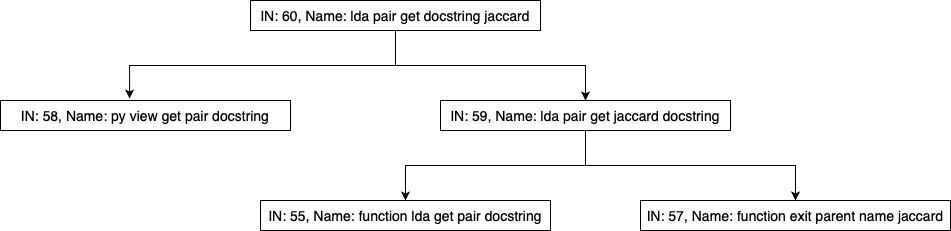
\includegraphics[width=1\columnwidth]{figures/hla2/rq1_hla1.png}
  \caption{Snippet from subject system 1 (Our code)}~\label{fig:rq1_hla1}
\end{figure*}

\subsection{ \textbf{RQ1: Effectiveness of word variation labeling}}
To see the effectiveness of labeling, we manually picked the root node and its neighborhood. We explored a similar tree snippet for the three systems. In Figure \ref{fig:rq1_hla1}, we see root node 60 has the label \textit{lda pair get docstring jaccard}. From this label, one can guess that something related to docstring, jaccard distance, and topic modeling LDA occurs in the higher\_level\_abstraction subject system. An interesting thing to notice is that name of node 60 and 59 is the same. Although node 58, which is a child node of 60 has two new keywords py and view that indicate something related to Python file and view occurs inside the nodes' execution paths. On the other hand, if we see the name for node 60 using TFIDF method variant( \textit{pretty\_print\_leaf\_node bfs\_with\_parent mining\_sequential\_patterns id\_to\_sentence cluster\_view}) , we see that using method as unit for TFIDF is more comprehensible than using word as unit for TFIDF. Another benefit of TFIDF method variant is for node 60 and 59, it provides different names according to their execution paths. On the other side, the word variant of TFIDF gives the same name for node 60 and 59 because of over\-fitting. 

\begin{figure*}[tb]
  \centering
  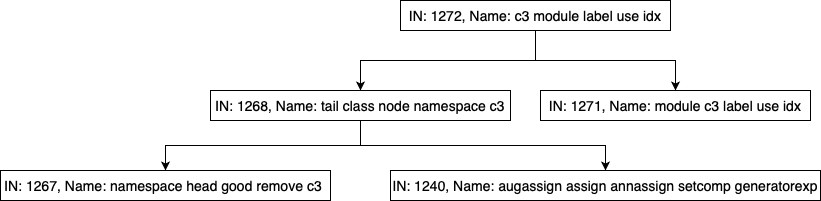
\includegraphics[width=\columnwidth]{figures/hla2/rq1_pyan1.png}
  \caption{Snippet from subject system 2 (pyan)}~\label{fig:rq1_pyan1}
\end{figure*}

In figure \ref{fig:rq1_pyan1} shows that we have a snippet of the Pyan subject system's abstraction tree. Pyan~\cite{pyan} is an open-source software which can extract call graph from a Python project. From our general knowledge, we can expect the concepts related to source code. If we look at node 1272 at Figure \ref{fig:rq1_pyan1}, the name is \textit{c3 module label use idx}. Except for the module, other keywords are not that much expressive. For node 1268, we see keywords like class, node, namespace indicate that the node is relevant to processing source code. However, we can see a recurrent occurrence of the same name for node 1272, 1271, which is an over-fit situation. Name for node 1272, 1271 using method variant TFIDF are 
\textit{write\_edge  find\_filenames  DotWriter}, \textit{write\_edge TgfWriter DotWriter visit\_Assign}  which clearly indicates some hint what the nodes do. 

In Figure \ref{fig:rq1_realTime1}, we have a snippet from our third subject system (Real-Time-Voice-Cloning \cite{realTime}). This open-source project can clone someone's voice from a clip of at least five seconds. So, this system's high-level functionalities can be converting wave length, processing audio, training model. The name of root node 806 is \textit{synthesize train synthesizer synthesize toolbox}. Here, train indicates training models, synthesize means processing audio signal, and toolbox indicates the tool system. For node 791, we see keywords like encoder, spec which indicates processing of signals. Using method name variant of TFIDF the name for node 806 and 791 are \textit{save\_wav encoder.audio discretized\_mix\_logistic\_loss profile\_noise encoder.visualizations}, \textit{current\_encoder\_fpath make\_spectrogram load\_preprocess\_wav normalize\_volume}. TFIDF method variant provides more contextual information from the name of node 806, 791. 

From the above manual investigation of node names using the method and word variant, it is evident that using method name variant provides more semantic abstraction. However, word variant provides a fixed-length  name. Yet, the output is ambiguous. So, We would recommend using method variant TFIDF to name or label an abstractio node.


\begin{figure*}[tb]
  \centering
  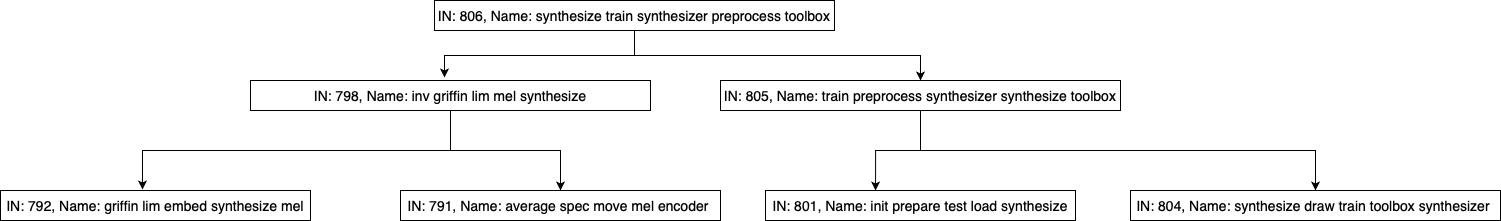
\includegraphics[width=\columnwidth]{figures/hla2/rq1_realTime1.png}
  \caption{Snippet from subject system 3 (Real-Time-Voice-Cloning)}~\label{fig:rq1_realTime1}
\end{figure*}



\subsection{ \textbf{RQ2: Natural text summary for abstraction nodes}} 
 Natural text is more comprehensive than a few keywords. Therefore, to support abstraction nodes' comprehension in a hierarchical tree, we propose to summarize the methods' docstring in all execution paths of the node. To keep the importance of each method, we used only the first line of the docstring. Also, from our manual analysis, it is evident that most of the time, the first line describes the function's purpose. Although for many cases, we found that docstring is absent. In those cases, we just omitted the method for generating summary. To answer our RQ2, we investigated the summary for nodes in three subject systems. 
 
 The root node 60 of subject system 1 has the text summary \textit{clustering execution paths using scipy Labeling a cluster using six variants  This function returns function name with their docstring  analyzing Python programs to build cluster tree of execution paths.} Subject system 1 is our program to cluster execution paths from a call graph. Then, we labeled the nodes in cluster using six different techniques and also analyzed docstring to produce summary that we discussed in this research question. If we carefully observe the summary for node 60, using TextRank algorithm our produced summary is almost accurate about what the first subject system does. For node 57, our approach's summary is \textit{converting tgf file to a networkX graph extracting function names from TGF file analyzing Python programs to build cluster tree of execution paths.} From the summary, we can confidently tell that abstraction node 57 deals with extracting function names from TGF file, converting TGF format file to networkX graph.
 
 
The root node 1272 of subject system 2 (Pyan) has the summary \textit{Resolve those calls to built-in functions whose return values Return a label for this node, suitable for use in graph formats.} As Pyan deals with source code, we can see the summary is saying something about resolving built-in functions, labeling nodes for graph format. We can relate this summary to the purpose of Pyan partially. For node 1271, the summary is \textit{Try to determine the full module name of a source file, by figuring out       Return the node representing the current class, or None if not inside a class definition.}
The summary for node 1271 says that the execution paths it abstracted mostly deal with determining a source file module, getting the class name a node represents. These are some standard utilities for a project which process source code. The summary for node 58 is \textit{Generate cluster figure from a dendrogram. Flattens a nested list. This function returns function name with their docstring.} Node 58 deals with plotting the dendrogram, mapping function name to docstring.

The root node 806 of subject system 3 (Real-Time-Voice-Cloning) has the summary \textit{If this function is not explicitely called, it will be run on the Args:                  Computes where to split an utterance waveform and its corresponding mel spectrogram to obtain   Derives a mel spectrogram ready to be used by the encoder from a preprocessed audio waveform.} As we have described previously, Real-Time-Voice-Cloning software can clone a voice to produce speech from text. If we see the summary generated by TextRank for node 806, we can say it deals with processing audio wave-forms. Furthermore, for node 801, the summary is \textit{Args:   Synthesizes mel spectrograms from texts and speaker embeddings.} Summary for node 801 is very small. It indicates that mostly docstring for Real-Time-Voice-Cloning is empty, and the short summary indicates text to speaker embedding, which is essential for voice cloning.

From the observation of node summary generated by TextRank for three subject systems, we can conclude that if functions are properly documented with docstring this approach can complement the comprehensiveness of abstraction nodes. We faced the challenge of different formats of comments, which hampered the extraction of the docstring. 

\subsection{ \textbf{RQ3: Effectiveness of mined patterns from execution paths}}
From our manual investigation into the execution paths of an abstracted node, we find that there are recurrent patterns that can help comprehend the abstracted node. Therefore, we develop a technique to use sequential pattern mining for selecting patterns among the execution paths from those findings. 

The patterns for root node 60 of subject system 1 are

\begin{itemize}
    \item ClusteringCallGraph,python\_analysis,clustering\_using\_\\
    scipy
    \item ClusteringCallGraph,python\_analysis,clustering\_using\\
    \_scipy ,labeling\_cluster
    \item ClusteringCallGraph,python\_analysis,clustering\_using\_\\scipy,
labeling\_cluster, tf\_idf\_score\_for\_scipy\_cluster
\end{itemize}
From observing this pattern, we can clearly tell that node 60 is working with Python code, clustering using scipy library, labeling the clusters. As this is the root node of the subject system 1, we can conclude the patterns clearly represent the root nodes purpose.

The patterns for node 58 are 

\begin{itemize}
    \item ClusteringCallGraph,PlayingWithAST
    \item ClusteringCallGraph,get\_all\_method\_docstring\_pair\_of\_a\_\\
    project
    \item ClusteringCallGraph,get\_all\_method\_docstring\_pair\_of\_a\_\\
    project,get\_all\_py\_files
\end{itemize}
From the patterns for node 58 retrieved by sequential pattern mining, we can see it is extracting docstring from all Python files which is one of the important part for answering our RQ2. 

The patterns for root node 1272 are

\begin{itemize}
    \item get\_attribute
    \item resolve\_builtins,get\_attribute
    \item analyze\_binding,resolve\_builtins
\end{itemize}

From the list of patterns, we can see there is very little information. Although these patterns are for the root node, they are most frequent. Limiting the length of the minimum pattern can solve the problem. However, we can understand that getting attributes, analyzing bindings, and resolving built-ins is the most common concept for root node 1272.

The patterns for node 1240 are 
\begin{itemize}
    \item resolve\_builtins,resolve\_method\_resolution\_order,\\
    C3\_linearize,C3\_merge
    \item analyze\_binding,resolve\_builtins,resolve\_\\method\_resolution\_
    order,C3
    \_linearize,C3\_merge
    \item resolve\_builtins,resolve\_method\_resolution\_order,\\
    C3\_linearize,C3\_merge,C3\_find\_good\_head,\\LinearizationImpossible
\end{itemize}
From the patterns of node 1240, we can see that method resolution order, linearize, resolve builtins are the main task.

The patterns for root node 806 of subject system 3 are

\begin{itemize}
    \item init,setup\_events
    \item wav\_to\_mel\_spectrogram
    \item embed\_utterance
    \item train
\end{itemize}

From the patterns for node 806, we see that it is creating different events, converting wave to spectrogram, and training model, which summarizes what Real\-Time\-Voice\-Cloning does. 
The patterns for node 804 are

\begin{itemize}
    \item wav\_to\_mel\_spectrogram
    \item encoder\_preprocess
    \item embed\_utterance
    \item encoder\_preprocess,\_preprocess\_speaker\_dirs,\\
    preprocess\_speaker
\end{itemize}
From the patterns of node 804, we can say that node 804 is embeddeing and encoding audio signals, prepossessing speaker audios.

From observing significant patterns of different nodes from three subject systems, we can conclude that providing them with an abstraction node can enhance a node's comprehensibility. However, the minimum length of each pattern and removing frequency-based bias should be considered to improve the patterns.
\subsection{ \textbf{RQ4: Effectiveness of using label, summary and patterns together}}

In RQ1, we manually analyzed how expressive the label for nodes using word and method variants. We found that method variation of the TFIDF technique provides a more sophisticated label than its word variant, which seems ambiguous. From our analysis of RQ2, we have seen promising summary for nodes using TextRank. Although this method's success hugely depends on how well the method docstring is written, excluding unrelated information is a challenge due to different formations. From RQ3, it is clear that patterns from execution paths are helpful to support nodes, although effectiveness hugely depends on selecting tuning mining pattern algorithms. Therefore, if the challenges for generating name, summary, and patterns are solved accordingly, they will enrich the comprehension of the abstraction node, in total, the overall hierarchical abstraction tree. 

\section{Threats to validity}

We have picked three different subject systems of varying size so that our approach's effectiveness can be generalized to some extent. We manually analyzed the results of our techniques to reach a saturated decision. Furthermore, two of the authors of this paper individually analyzed the findings to remove subjective biases. We carefully picked the first line skipping lines with special characters to extract the docstring for each method. 
\section{Related Work}
\label{related}
\subsection{Program Comprehension in general}
Program comprehension is a cognitive way of understanding software systems to perform different software maintenance tasks \cite{wei2002surveyCategorizationComprehension, siegmund2016programPastFuture}. Three different type of cognitive models \cite{tilley1998reverseEngineeringFramework, von1993programToolRequirements, siegmund2016programPastFuture} can be found in the literature which is followed consciously or unconsciously by developers. The comprehension models are Top-down, Bottom-up, and Integrated. When developers have prior domain knowledge about a software system, the top-down model is preferred as they can map domain knowledge to low-level source code hierarchically \cite{brooks1983theoryComprehensionPrograms}. On the other hand, when developers lack domain knowledge, they start with low-level source code and then group the functionality together to have a hierarchical abstraction of the system features \cite{shneiderman1979syntacticInteractionsModel, pennington1987stimulusMentalRepresentations}. Integrated model \cite{shaft1995relevanceDomainKnowledge, von1993programToolRequirements} is a mix of top-down and bottom-up approach. The problem in hand and the target system have different properties in the real world, which demand switching between top-down and bottom-up models. Generally, a developer can have prior domain knowledge of a few portion and point-blank for the rest of the system. This situation deserves the adapted use of both top-down and bottom-up approaches.   


\subsection{IR techniques to Name source code artifacts}
% \cite{mcburney2014improvingTopicSummarize}
% \cite{de2012IRMethodsArtifacts} \cite{panichella2013topicModelsTasks}
% \cite{chen2016topicMiningRepositories}
% Very very important \cite{sun2016surveyTopicSE}
As software repositories contain unstructured data, topic model techniques are widely applied for different software engineering tasks to retrieve information \cite{chen2016topicMiningRepositories, panichella2013topicModelsTasks, sun2016surveyTopicSE}. Most common tasks where topic models showed promising results are source code comprehension, feature location, refactoring, bug localization, and others \cite{sun2016surveyTopicSE}. Lucia et al. \cite{de2012IRMethodsArtifacts} conducted a study to see how information retrieval techniques perform compared to manual naming Java class files. Developers were asked to pick ten keywords for each class file, and top-10 words are picked using different topic model technique and custom heuristics. Their experiment shows that in 40\%-80\% cases, automatic and human label overlaps. 

\subsection{Reverse Engineering}

\subsubsection{Subsystem Identification}
Muller et al. \cite{muller1990composingSubsystemStructures} proposed subsystem detection algorithm using different clustering components like variable, procedure, and modules. 
According to Bass et al. \cite{bass2003softwareArchitecturePractice}, two types of software architecture are useful for understanding a complex software system. They are Conceptual and Concrete architecture. A conceptual architecture provides high-level abstraction skipping the code level details. On the other hand, concrete architecture shows the implementation level information. Roy et al. \cite{roy2008softwareArchitectureRecovery} propose and evaluate a framework for the incremental and iterative application of automated architecture recovery (using SWAG Kit) and architecture analysis (using SAAM.). They showed that the reverse engineering tool cannot recover a deeply understood conceptual architecture without SAAM's application but can create a reasonable basis towards that direction. Murphy et al.\cite{MurphyNotkin2001} show that by generating reflexion models from high-level model and source model (i.e., static call graphs), it is possible to facilitate program understanding to the novice developers. 

In this study, we try to automatically recover conceptual architecture from concrete architecture, reducing manual effort.

\subsubsection{Call graphs to abstract a software system behaviors}
Static and dynamic call graphs are used in literature to help developers comprehend a software system to aid different maintenance tasks \cite{feng2018hierarchicalExecutionComprehension, gharibi2018automaticStaticCluster, xin2019identifyingFeaturesExecution}. Feng et al. \cite{feng2018hierarchicalExecutionComprehension} proposed an approach to use dynamic call graphs for understanding a system's behavior. They instrumented the subject systems to generate execution traces of method entry and exit events. Later, they followed the duplication removal process and constructed a call graph from the execution traces. Execution phases from this dynamic call graph are clustered to get system behaviors. Similarly, Gharib et al. \cite{gharibi2018automaticStaticCluster}, and Vijay et al. \cite{walunj2019graphevoEvolutionCall} also adopted clustering of execution paths from call graphs of the static variant. Using a static call graph brings the benefit of capturing all possible scenarios and less redundant data to handle than dynamic call graph \cite{gharibi2018automaticStaticCluster}. 

\subsubsection{IR techniques on the hierarchical abstraction of software system}
Feng et al. \cite{feng2018hierarchicalExecutionComprehension} proposed an approach to identify behaviors of a system by hierarchically abstracting dynamic call graph from execution traces. Sequential pattern mining is applied to mine significant portions from the execution phases. Hierarchical clustering is performed to group execution phases. Later, the clusters are labeled using the Tfidf score, where method signatures serve as terms and the phases as document. 
Paul et al. \cite{mcburney2014improvingTopicSummarize} used static call graph to hierarchically abstract a system. In their hierarchical view, each node represents a method. To mine the topics, keywords from methods are considered. Hierarchical Document Topic Model (HDTM) by \cite{weninger2012documentTopicHierarchies} Weninger et al. is adopted, which works on graph documents to mine topic. Gharib et al. \cite{gharibi2018automaticStaticCluster} took a different approach. They went further with the static call graph by extracting execution paths and then clustering the execution paths. Each cluster in the cluster tree is labeled using top-5 method names from Tfidf. Levy et al. \cite{levy2019understandingLargeHierarchical} found interviewing developers that two kinds of comprehension go for large scale hierarchical view. They are system comprehension and code comprehension. In this paper, we tried to adopt static call graph analysis from Gharib et al. and then improve their labeling technique. Nodes of the cluster tree is considered as a behavioral abstraction unit of a system. Method comments are used to generate a description of the unit and sequential pattern mining to create sample examples. 
\section{Conclusion and Future Plan}
In software engineering, program comprehension is an important research area that involves many other software maintenance tasks. Nowadays, the size and complexity are growing. To perform a maintenance task, developers need to understand how different components of the system interact. Other cognition models are studied in the literature to aid developers. Top-down and bottom-up models are popular program comprehension models. In these models, developers map high-level features with low-level implementations depending on a specific situation. Different hierarchical abstraction techniques which use call graph of dynamic and static variation exists. 

This study focused on improving a software system's abstraction hierarchically using execution paths from a static call graph. Executions paths represent low-level implementation. Grouping execution paths in a cluster tree, a software system is hierarchically abstracted. Information presented with the nodes of a cluster tree is useful for developers to map high-level features to low-level implementations. We proposed different techniques like using word and method variant for TFIDF to label nodes, generated summary for each node from method docstring, and mined significant patterns to attach all these three types of information with each node to aid comprehension.

To evaluate our approach, we conducted an exploratory case study to determine our proposed techniques' effectiveness. We discussed the generated output for different nodes and challenges to improve. We found that generalizing the techniques with more subject system would improve the techniques. In the future, we plan to use source code summarizing techniques to produce more accurate summary. Moreover, we plan to build an automated tool that, given a software system (Python), will produce a hierarchical abstraction tree that developers can browse interactively. We have a plan to conduct a wide-scale user study to evaluate these techniques.
